\documentclass{beamer}
%pacchetti
\usepackage[T1]{fontenc}
\usepackage[utf8]{inputenc}
\usepackage{graphicx}
\usepackage[italian]{babel}
\usepackage{mathrsfs}
\usepackage{booktabs}
\usepackage{amsmath}
\usepackage{amsfonts}
\usepackage{amssymb}
\usepackage{amsbsy}
\usepackage{amsthm}
\usepackage{enumerate}
\usepackage{quoting}
\quotingsetup{font=small}
\usepackage{diagbox}
\usepackage{graphicx}
\usepackage{setspace}
\usepackage{float}
\usepackage{version}
\usepackage{multicol}
\usepackage{beamerfoils}

\usepackage[none]{hyphenat} %avoid hyphenation
\usepackage{xcolor} %to uset \textcolor
% end pacchetti

\usetheme[bgphoto]{polimi}

% Full instructions available at:
% https://github.com/elauksap/beamerthemepolimi

% Set custom font (requires to compile with XeLaTeX).
\usepackage{ifxetex}
\ifxetex
\usepackage{fontspec}
\setsansfont[Scale=0.6]{Arial}
\fi

\usepackage{lipsum}


\newcommand\mynum[1]{%
	\usebeamercolor{enumerate item}%
	\tikzset{beameritem/.style={circle,inner sep=0,minimum size=2ex,text=enumerate item.bg,fill=enumerate item.fg,font=\footnotesize}}%
	\tikz[baseline=(n.base)]\node(n)[beameritem]{#1};%
}


\title{{\LARGE Is Dementia predictable?}}

%\subtitle{Subtitle}
\author{F. Di Filippo, E. Manfrin, E. Musiari, E. Palli}
\date{17 december 2021}



\begin{document}
	
	\begin{frame}
		\maketitle
	\end{frame}



\begin{frame}{Our team}
\begin{minipage}{0.24\textwidth}
	\vspace{0.55cm}
	\begin{center}%
		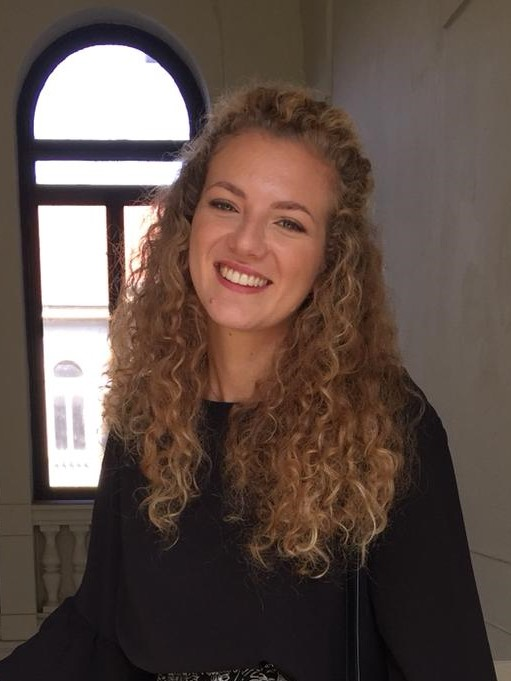
\includegraphics[width=\columnwidth]{francescataglio.jpeg}
		Francesca Di Filippo
	\end{center}
\end{minipage}
\hfill
\begin{minipage}{0.24\textwidth}
	\begin{center}%
		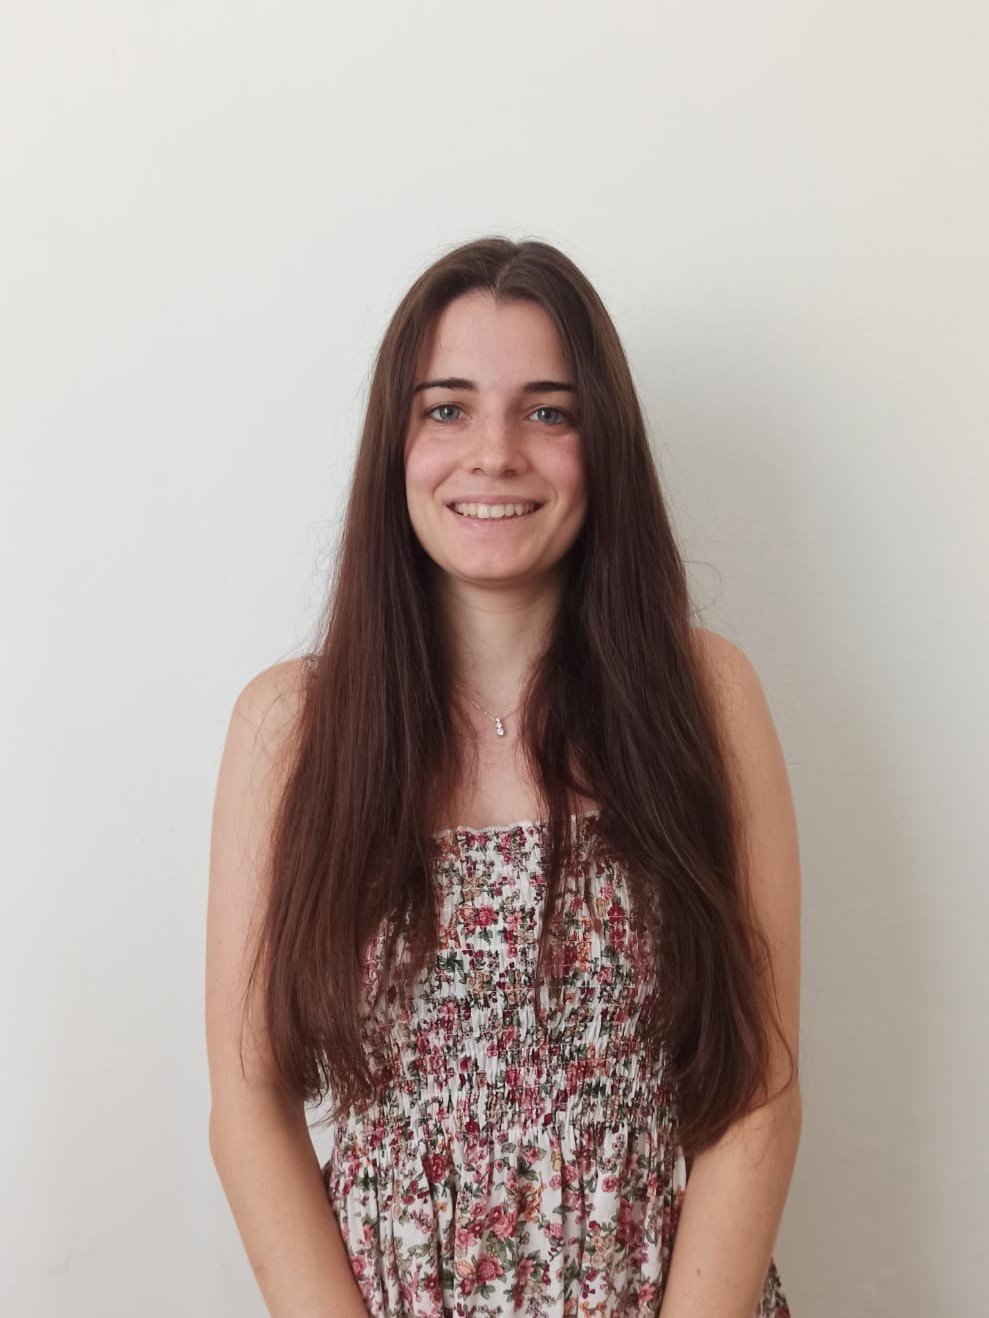
\includegraphics[width=\columnwidth]{erikataglio.jpeg}
		Erica Manfrin
	\end{center}
\end{minipage}
\hfill
\begin{minipage}{0.24\textwidth}
	\begin{center}%
		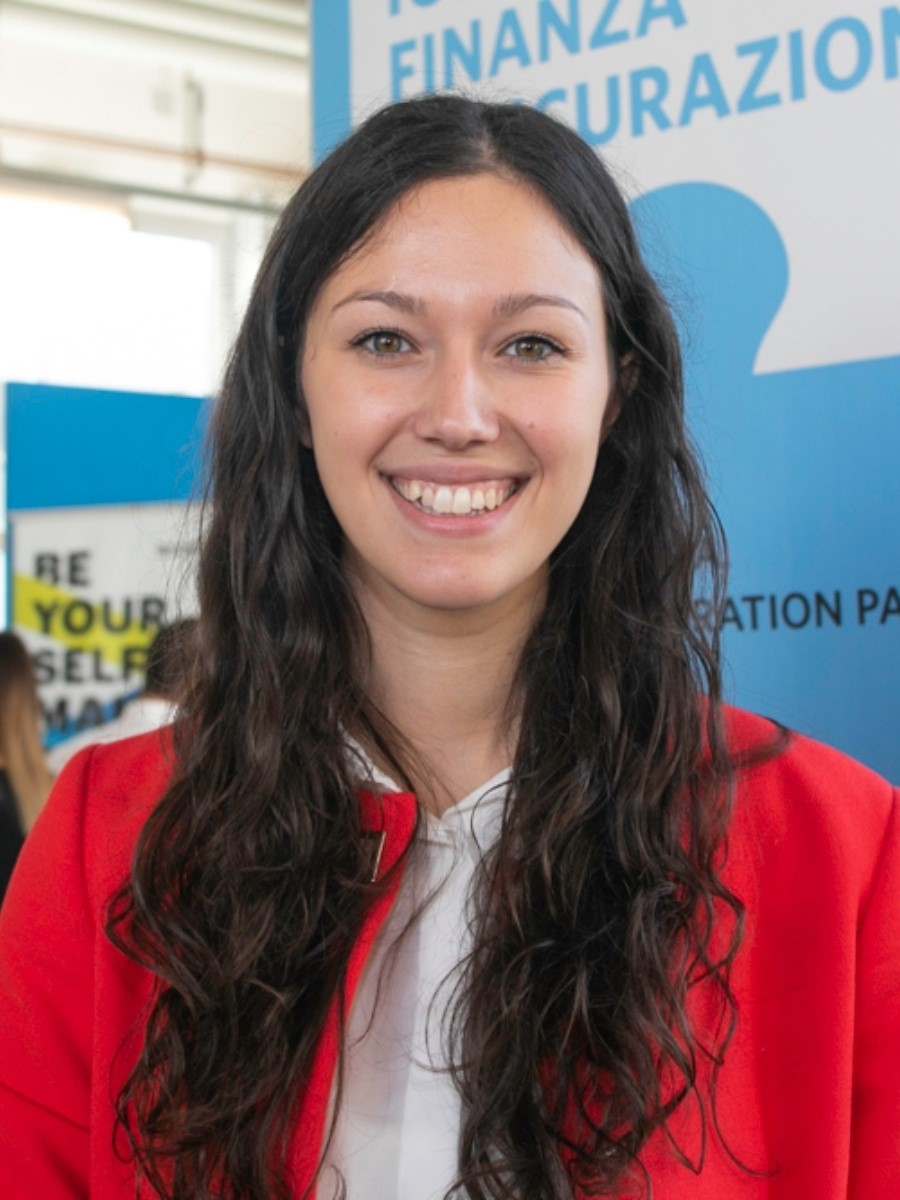
\includegraphics[width=\columnwidth]{elenataglio.jpg}
		Elena Musiari
	\end{center}
\end{minipage}
\hfill
\begin{minipage}{0.24\textwidth}
	\begin{center}%
		
\includegraphics[width=\columnwidth]{edoardotaglio.jpeg}
		Edoardo Palli
	\end{center}
\end{minipage}


\end{frame}

	
	
	\begin{frame}{Dataset}
		
		Dataset Dementia and Alzheimer longitudinal
		%\vspace{0.2 cm}
		\begin{center}
			
			
			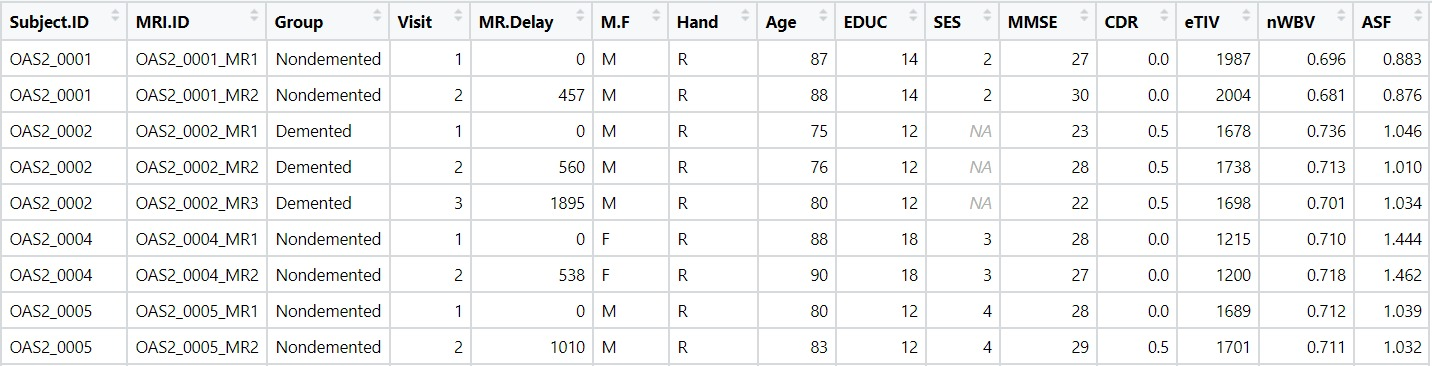
\includegraphics[width=\columnwidth]{dataset_al.jpeg}
		\end{center}
		
		
		where SES is Socioeconomic Status, MMSE is Mini Mental State Examination, CDR is Clinical Dementia Rating, eTIV is Estimated Total Intracranial Volume, nWBV is Normalize Whole Brain Volume and ASF is Atlas Scaling Factor.
		
		\vspace{0.1 cm}
		Source: Kaggle
		
		
	\end{frame}
	
	
	
	\begin{frame}{Analysis Male VS Female}
		%VARIABLE TAKEN INTO CONSIDERATION
		\vspace{0.1cm}
	
	\begin{small}	Variable considered: $[Age,EDUC,MMSE,eTIV,nWBV,ASF]$ \end{small}
		\vspace{-0.2cm}
		
	$$
	H_0: \mathbf{Y}_{female} \overset{d}{=} \mathbf{Y}_{male}\;vs\;H_1:\mathbf{Y}_{female} \overset{d}{\neq} \mathbf{Y}_{male}
	$$
	 
	% hist: histmvsf
	
	\begin{multicols}{2}
		
	\vspace{0.5cm}
	$T_0 = |\bar{Y}_{female} - \bar{Y}_{male}|$	
	
	\vspace{1cm}
	$pvalue= 0 $
	\columnbreak

	\begin{center}
		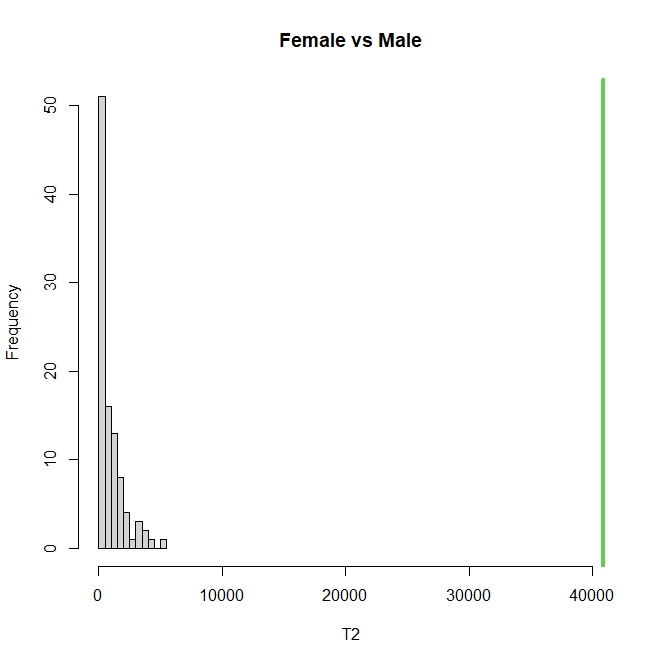
\includegraphics[width=0.95\columnwidth]{histmvsf.jpeg}
	\end{center}
	\end{multicols}
	% pvalue: non mi viene la linea verde

	
	\end{frame}


	\begin{frame}{Demented VS Nondemented }
	\vspace{-0.3cm}
		$$
	H_0: \mathbf{Y}_{Demented} \overset{d}{=} \mathbf{Y}_{Non Demented}\;vs\;H_1:\mathbf{Y}_{Demented} \overset{d}{\neq} \mathbf{Y}_{Non Demented}
	$$
	
 	% hist: histdemvsnondem
 	% pvalue:  histdemvsnondem
 	\begin{center}
 		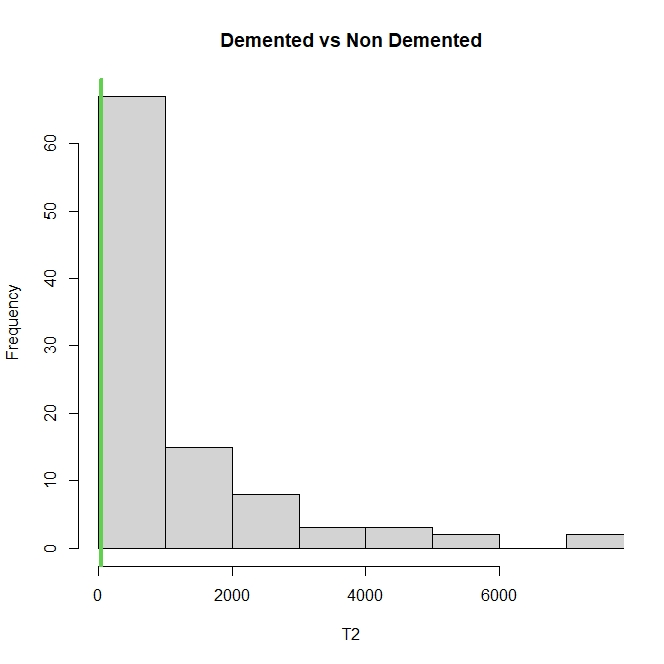
\includegraphics[width=0.5\columnwidth]{histdemvsnondem.jpeg}
 	\end{center}
 	\vspace{-0.7cm}
 	$pvalue= 0.9 $
	\end{frame}
	
	\begin{frame}{Demented VS Nondemented only Male}
	\vspace{-0.3cm}
	$$
	H_0: \mathbf{M}_{Demented} \overset{d}{=} \mathbf{M}_{Non Demented}\;vs\;H_1:\mathbf{M}_{Demented} \overset{d}{\neq} \mathbf{M}_{Non Demented}
	$$
		% hist: histdvsnmale
	% pvalue: pvaluedvsnmale
	\begin{center}
		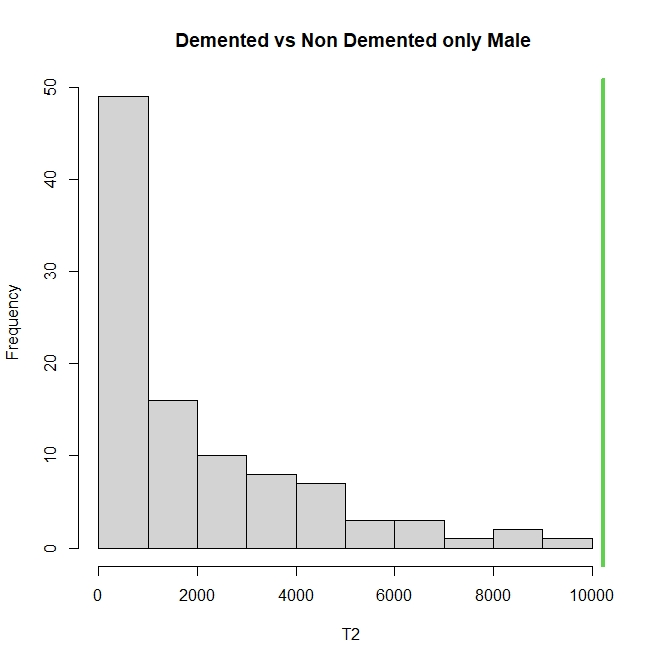
\includegraphics[width=0.5\columnwidth]{histdvsnmale.jpeg}
	\end{center}
	\vspace{-0.7cm}
	$pvalue= 0 $
	\end{frame}
	
	\begin{frame}{Demented VS Nondemented only Female}
	\vspace{-0.4cm}
	$$
	H_0: \mathbf{F}_{Demented} \overset{d}{=} \mathbf{F}_{Non Demented}\;vs\;H_1:\mathbf{F}_{Demented} \overset{d}{\neq} \mathbf{F}_{Non Demented}
	$$
	% hist: dvsnfemale
	% pvalue: pvaluedvsnfemale
	\begin{center}
		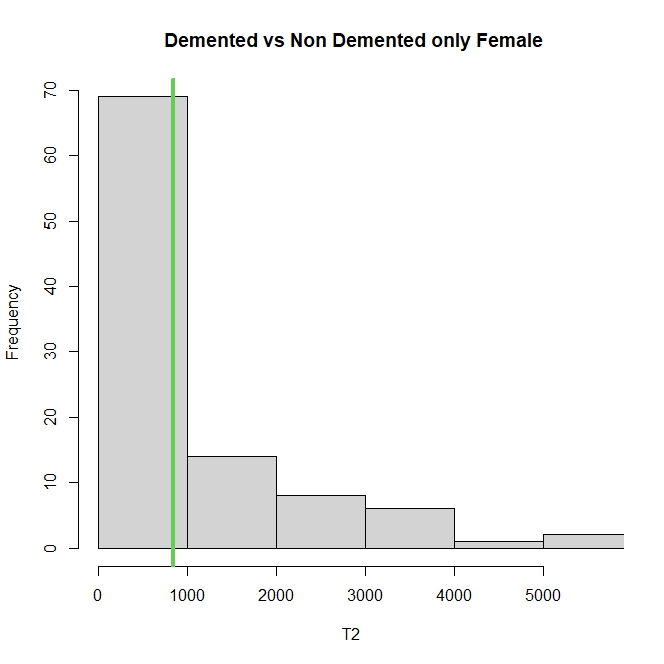
\includegraphics[width=0.5\columnwidth]{dvsnfemale.jpeg}
	\end{center}
	\vspace{-0.7cm}
	$pvalue= 0.37 $
		
	\end{frame}
	
	
	\begin{frame}{ TWO WAYS ANOVA: EDUCATION (I)}
	\vspace{-0.3cm}
 	$$ EDUC =   \mu + \alpha_i + \beta_j + \gamma_{ij} + \epsilon  $$
 	$ j =\{male,female\} \;$,
 	$\: i=\{ Demented, Non Demented \}$
 	
 	
 	$\: \alpha= sex \space$, 
	$\: \beta= diagnostic \space$, 
	$\: \gamma= interaction$
	$$
	H_0: \gamma_{ij}=0\; \;vs\;H_1:\gamma_{ij}\neq0 
	$$
	TEST STATISTIC: $ T0= F-STATISTICS \; $
	
	$\; p-value = 0.082 $
	at level of confidence $ 95\% $ there's no evidence to	reject $H_0$, 
	so we reduce the model
	\vspace{-0.2cm}
	
	
\end{frame}
	
\begin{frame}{TWO WAYS ANOVA: EDUCATION (II)}

	$$ EDUC =  \mu + \alpha_i + \beta_j  + \epsilon $$
	$$
	H_0: \beta_j=0\; \;vs\;H_1:\beta_i\neq0 
	$$
	$p-value = 0.069$
	at level of confidence $ 95\% $ there's no evidence to	reject $H_0$ 
	
	$$ EDUC =  \mu + \alpha_i  $$
	
		$$
	H_0:\alpha_i=0\; \;vs\;H_1:\alpha_i\neq0
	$$
	$p-value = 0.08 $
we could say that's neither of the grouping is significant at $95\%$ 

while with parametric test at least the diagnostic division is significant
\end{frame}
	\begin{frame}{ TWO WAYS ANOVA: MMSE (I)}
	$$ MMSE =   \mu + \alpha_i + \beta_j + \gamma_{ij} + \epsilon $$
		$ j =\{male,female\} \;$,
	$ i=\{ Demented, Non Demented \}$
	$$
	H_0: \gamma_{ij}=0\; \;vs\;H_1:\gamma_{ij}\neq0 
	$$
	
	TEST STATISTIC: $ T0= F-STATISTICS \;$
	
	$\; p-value = 0.875 $
	
	there's no evidence to	reject $H_0$,  
	so we reduce the model
	
	
\end{frame}

\begin{frame}{TWO WAYS ANOVA: MMSE (II)}

	$$ EDUC =   \mu + \alpha_i + \beta_j  + \epsilon  $$
	$$
	H_0:\beta_j=0\; \;vs\;H_1:\beta_j\neq0 
	$$
	
	$p-value = 0.446$
	there's no evidence to reject $H_0$
	
	$$ EDUC =  \mu + \alpha_i $$
	
	$$
	H_0: \alpha_i =0\; \;vs\;H_1:\alpha_i \neq0 
	$$
	$p-value = 0$
	there's evidence to reject $H_0 $ 
	so the most significative model is $ MMSE \sim Diagnostic$
	where Diagnostic is the division between Demented and Non Demented
	\end{frame}



	
	\begin{frame}{Regression}
	
	\vspace{0.3cm}
		
		% modello logistico e spiegare: demented and non demented e le covariate usate: ses, normal brain volume, age, mmse -> smoothing splines; cdr senza smoothing perchè pochi valori distinti
		% fittato su tutto il dataset esclusi i converted
		
		% summary, shapiro e qqplot
		
		Used a logistic model of classification Demented-Nondemented, with smoothing splines (degree 3) for EDUC, nWBV, Age, MMSE
		
		$$ \log \frac{p}{1-p} = EDUC + nWBV + Age + MMSE + CDR$$
		
		\vspace{0.2cm}
		with $p =$ probability that the observation is 'Demented'
		
	%	\begin{multicols}{2}
	
	
		\begin{center}
			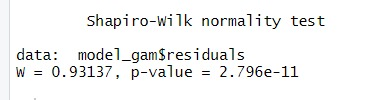
\includegraphics[width=0.6\columnwidth]{regr1.jpeg}
		\end{center}
	%	\columnbreak
	%	\begin{center}
	%		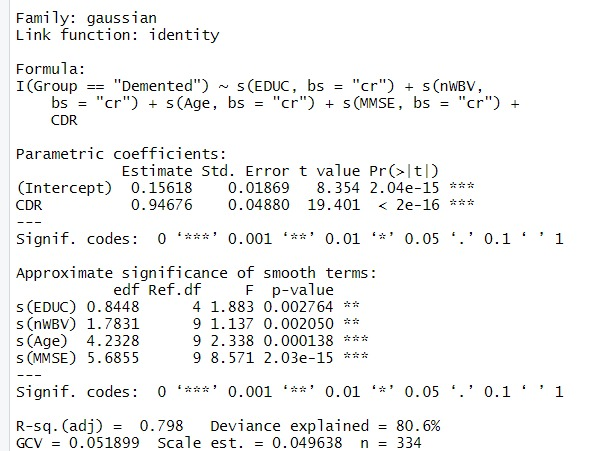
\includegraphics[width=\columnwidth]{regr2.jpeg}
	%	\end{center}
	%	
	%	\end{multicols}
		
		
	\end{frame}
	
	\begin{frame}{Prediction}
	
	Prediction for Converted patients:
	\begin{center}
		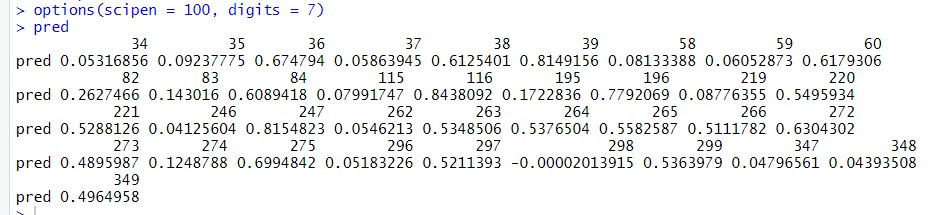
\includegraphics[width=\columnwidth]{prediction.jpeg}
	\end{center}

	Prediction for Nondemented patients:
	\begin{center}
		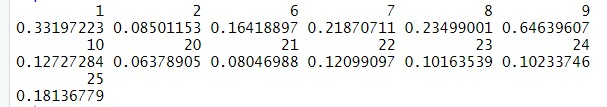
\includegraphics[width=0.8\columnwidth]{prediction2.jpeg}
	\end{center}	

		
	\end{frame}

	\begin{frame}{Survival Analysis (I)}
		
		\vspace{0.3 cm}
		Event: disease occurred
		
		\begin{center}
			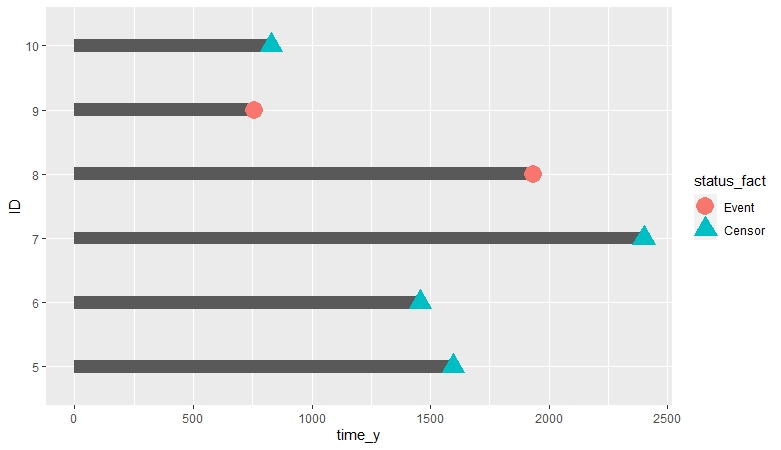
\includegraphics[width=0.9\columnwidth]{survival_plot2.jpeg}
		\end{center}
	\end{frame}

	\begin{frame}{Survival Analysis (II)}
	
		\begin{center}
			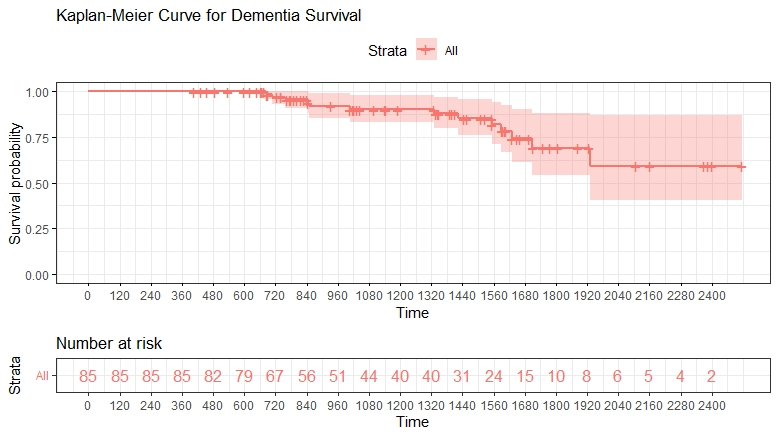
\includegraphics[width=\columnwidth]{kaplan-meier_bello.jpeg}
		\end{center}
	\end{frame}

	\begin{frame}{Survival Analysis(III)}
	
		\begin{center}
			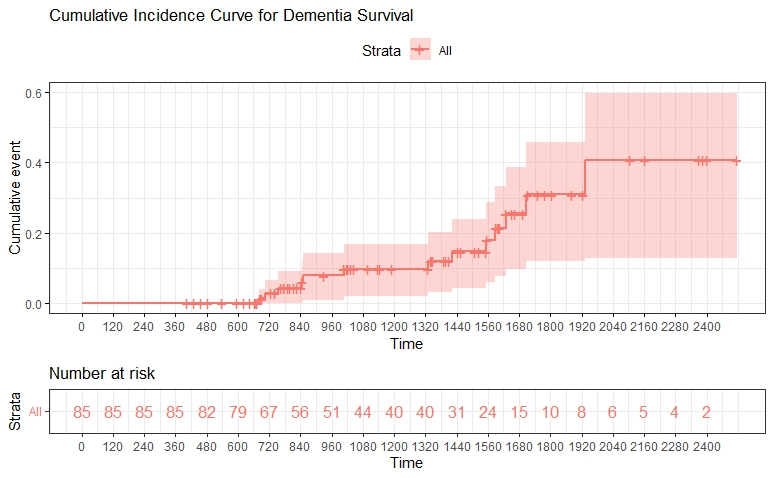
\includegraphics[width=0.95\columnwidth]{cumulative.jpeg}
		\end{center}
	\end{frame}


	\begin{frame}{Survival Analysis - Balanced (I)}
	
		\begin{center}
			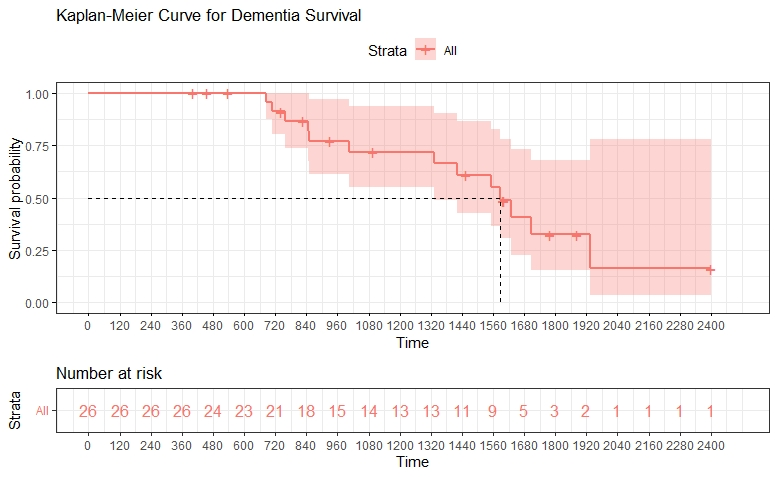
\includegraphics[width=\columnwidth]{kaplan-meier_bilanciati.jpeg}
		\end{center}
	\end{frame}
	
	\begin{frame}{Survival Analysis - Balanced (II)}
	
		\begin{center}
			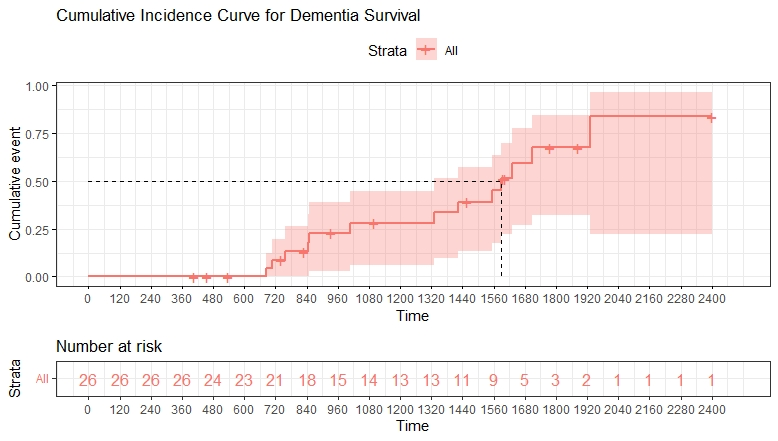
\includegraphics[width=\columnwidth]{cumulative_bilanciati.jpeg}
		\end{center}
	\end{frame}

	
	\begin{frame}{Future goals}
	
	\begin{itemize}
		\item Complete our survival analysis
		\item Solve the residual gaussianity problem
		\item Perform a prediction on the other dataset of patient (not labelled)
	\end{itemize}
		
	\end{frame}
	
	
\end{document}